\documentclass[12pt,a4paper]{article}

\newcommand{\TETELNUMBER}{10}
\newcommand{\TETELTITLE}{Turing-gép, RAM-gép, Boole-függvények és logikai hálózatok}
\newcommand{\TETELSHORTTITLE}{Számítási modellek}

\newcommand{\ZVTetelsorDataOnly}{}
\newcommand{\ZVTetelOne}{Adatok, adattípusok, adatműveletek és adatstruktúrák. Szám adattípus. Számrendszerek, konverziók. A logikai, halmaz, karakter, sztring absztrakt adattípusok és realizációjuk. A tömb (vektor, mátrix), rekord absztrakt adattípusok.}
\newcommand{\ZVTetelTwo}{Az algoritmus. Iteratív és rekurzív algoritmus. A számítógépes memória. Adat és program. Verem és procedúra. Az algoritmus lejegyzése. A folyamatábra és a pszeudokód. Elemi algoritmusok.}
\newcommand{\ZVTetelThree}{Strukturált programozás. Programgráf, valódi program, vezérlőgráf lebontása, strukturált program és annak formulája. Strukturált programgráf kialakítása, struktogram. Ciklikus bonyolultság és egyéb bonyolultsági tételek.}
\newcommand{\ZVTetelFour}{Számelméleti algoritmusok. Legnagyobb közös osztó, euklideszi és kibővített euklideszi algoritmus, lineáris kongruencia egyenletek. Multiplikatív inverz, moduláris hatványozás, Fermat prímteszt. RSA.}
\newcommand{\ZVTetelFive}{Rendezések: Beszúró rendezés. Az ,,Oszd meg és uralkodj!'' elv. Összefésülő rendezés. Gyors rendezés. Buborék rendezés. Shell rendezés. Minimum kiválasztásos rendezés. Négyzetes rendezés. Lineáris idejű rendezések: leszámláló rendezés, számjegyes rendezés. Időelemzéseik. Az összehasonlító rendezések időtétele.}
\newcommand{\ZVTetelSix}{Gráfalgoritmusok. Szélességi keresés. Mélységi keresés. Topologikus rendezés. Optimumfeladatok fákon (minimális feszítőfák, Kruskal- és Prim-algoritmus). Legrövidebb utak meghatározása (Dijkstra-algoritmus, Bellman--Ford-algoritmus, Floyd--Warshall-algoritmus).}
\newcommand{\ZVTetelSeven}{A párhuzamos algoritmusok alapfogalmai, PRAM modell, hatékonysági mértékek (munka, költség, gyorsítás, hatékonyság). Párhuzamos végrehajtás ábrázolási módjai. Komplexitás becslése, párhuzamos komplexitás. Amdahl törvénye. Pipeline párhuzamosítás, Lost update probléma bemutatása és megoldása.}
\newcommand{\ZVTetelEight}{Aggregáció, redukció, prefixszámítás párhuzamosítási lehetőségei. \texttt{CREW\_PREFIX}, \texttt{EREW\_PREFIX} és \texttt{OPTIMAL\_PREFIX} algoritmusok bemutatása. Összefésülő rendezés párhuzamosítási módja.}
\newcommand{\ZVTetelNine}{A busz, gyűrű, rács, tórusz, hiperkocka és fa topológiák bemutatása, csomópontok közötti távolságok jellemzése. A CSP, Publish--Subscribe és az Aktor modell. Az aszinkron programozás elemei: async, await kulcsszavak használata, coroutine-ok.}
\newcommand{\ZVTetelTen}{A Turing-gép fogalma, működése. A RAM-gép. Boole-függvények és logikai hálózatok.}
\newcommand{\ZVTetelEleven}{Algoritmikus eldönthetőség. Church-tézis. Rekurzív és rekurzívan felsorolható nyelvek, rekurzív illetve parciálisan rekurzív függvények. Nevezetes nyelvek (Az R, Re, coR, coRE nyelvosztályok és ezek kapcsolata) és bonyolultságuk. Algoritmikusan eldönthetetlen problémák. Polinomiális idejű algoritmusok.}
\newcommand{\ZVTetelTwelve}{Nemdeterminisztikus Turing-gépek, az NP és a coNP nyelvosztály. Példák NP-beli nyelvekre. A tanú-tétel. Nemdeterminisztikus algoritmusok bonyolultsága. NP-teljesség, Cook-tétel. Néhány NP-teljes probléma, Cook--Levin-tétel.}
\newcommand{\ZVTetelThirteen}{A Java programozási nyelv története, alapvető jellemzői. Egy Java program szerkezete (csomagok és fordítási egységek). Az objektumorientált programtervezés alapelveinek felsorolása. Objektumok tárolása és élettartama. Szemétgyűjtő mechanizmus. Kivételkezelés.}
\newcommand{\ZVTetelFourteen}{Az egységbezárás és az információrejtés objektumorientált alapelvek megvalósítása. Osztálydefiníció és példányosítás. Osztályszintű és példányszintű tagok, konstansok. Hozzáférési kategóriák és használatuk. Hivatkozás az osztály tagjaira.}
\newcommand{\ZVTetelFifteen}{Az öröklődés és a polimorfizmus objektumorientált alapelvek megvalósítása. Öröklődés szabályai, metódusok túlterhelése és felüldefiniálása. A referencia statikus és dinamikus típusa. Absztrakt osztály és interfész szerepe, összehasonlítása.}
\newcommand{\ZVTetelSixteen}{Az operációs rendszerbeli folyamat (processz) fogalma. Folyamatkontextus. A fonál (szál) fogalma. A processzállapotok, állapotváltások, processz futási módok. Taszk- és fonálállapotok, állapotátmenetek.}
\newcommand{\ZVTetelSeventeen}{A memóriamenedzselés feladatai. Memória mint erőforrás. Címleképzés fajtái. Lapozós virtuális memóriamenedzselés működése. Allokálás, nyilvántartás, címleképzés. Laphiba fogalma, kezelése, kilapozási stratégiák. Előnyök, hátrányok.}
\newcommand{\ZVTetelEighteen}{Fájlrendszer-megvalósítási feladatok. Jegyzékszerkezetek. Szabadblokk-menedzselési lehetőségek. Fájlattribútum-rögzítési lehetőségek (ezen belül a fájltestet képező blokkok rögzítési lehetőségei).}
\newcommand{\ZVTetelNineteen}{Relációs adatmodell, relációs struktúra és integritási feltételek. ER modell elemei jelentése és jelölése. Az ER modell konverziója relációs modellre. Relációs adatmodell műveleti része, relációs algebra.}
\newcommand{\ZVTetelTwenty}{Az SQL szabvány relációs adatbázis kezelő nyelv bemutatása, a DDL (objektum létrehozás, megszüntetés és szerkezet módosítás), DML (rekord felvitel, törlés és módosítás), DCL és a SELECT utasítások áttekintése és használata. Beágyazott SELECT használata. A relációs algebra műveleteinek megvalósítása SQL-ben.}
\newcommand{\ZVTetelTwentyOne}{Adatkezelés és adatbáziskezelés alapfogalmai, fileszervezési módszerek, B-fa index; adatbázis architektúra; A normalizálás szerepe a relációs adatbázis kezelésben. Redundancia oka és a megszüntetés lépései. Normálformák. Dekompozíció célja és szabályai, tételei.}
\newcommand{\ZVTetelTwentyTwo}{Számítógép-hálózatokhoz kötődő alapfogalmak és az ISO--OSI hivatkozási modell: topológia és méret szerinti osztályozásuk. Kapcsolástechnika szerinti osztályozásuk (vonalkapcsolás, üzenetkapcsolás, csomagkapcsolás és virtuális vonalkapcsolás). Az ISO--OSI hivatkozási modell szerkezete, rétegei és azok főbb funkciói.}
\newcommand{\ZVTetelTwentyThree}{A számítógép-hálózatok ISO--OSI hivatkozási modell adatkapcsolati rétegének közeghozzáférési alrétege: A főbb csatorna-megosztási osztályok (statikus-dinamikus, dinamikus versengő-determinisztikus) bemutatása és azok összevetése. Az IEEE 802.3 és az Ethernet (CSMA/CD) keretformátum, MAC címek, támogatott közegek és sebességek bemutatása, működés duplex csatorna esetén. Az IEEE 802.11 WLAN általános felépítése, az Access Point (AP) főbb funkciói. Az alkalmazott közeghozzáférési módszer (CSMA/CA), Distributed Coordination Function (DCF) és Point Coordination Function (PCF) üzemmódok.}
\newcommand{\ZVTetelTwentyFour}{A TCP/IP protokollszövet és az Internet. Az Internet hivatkozási modell (DoD) és az ISO--OSI hivatkozási modell összevetése. A TCP/IP protokollszövet főbb részei (ARP, RARP, IP, ICMP, TCP, UDP) és azok funkciói. Az internetes címzés és címosztályok: IPv4-címosztályok, maszk, subnet, supernet, osztály nélküli címzés (CIDR -- Classless Inter-Domain Routing) és változó alhálózat-méretek (VLSM -- Variable Length Subnet Mask), címek kiosztása, lokális címek és címfordítás (NAT). IPv6-címek, IPv6-címtípusok (unicast, multicast, anycast; link local, unique local, aggregatable global unicast address).}
\newcommand{\ZVTetelTwentyFive}{Szoftvertechnológia és a szoftverfolyamat fogalma. A szoftverfolyamat-fázisok részletes bemutatása: szoftverspecifikáció, tervezés, implementáció, validáció és evolúció. Az evolúciós modell ismertetése.}
\newcommand{\ZVTetelTwentySix}{Szoftverkövetelmény fogalma és osztályozásai. Követelmények általános problémái. Követelményfeltárás és -elemzés folyamata. Vezérlési stílusok.}
\newcommand{\ZVTetelTwentySeven}{UML diagramok bemutatása: Use case és osztálydiagram. A szekvenciadiagram. Komponensdiagram.}

\newcommand{\ZVTetelKiiras}[1]{%
  \ifcase#1\relax
  \or \ZVTetelOne
  \or \ZVTetelTwo
  \or \ZVTetelThree
  \or \ZVTetelFour
  \or \ZVTetelFive
  \or \ZVTetelSix
  \or \ZVTetelSeven
  \or \ZVTetelEight
  \or \ZVTetelNine
  \or \ZVTetelTen
  \or \ZVTetelEleven
  \or \ZVTetelTwelve
  \or \ZVTetelThirteen
  \or \ZVTetelFourteen
  \or \ZVTetelFifteen
  \or \ZVTetelSixteen
  \or \ZVTetelSeventeen
  \or \ZVTetelEighteen
  \or \ZVTetelNineteen
  \or \ZVTetelTwenty
  \or \ZVTetelTwentyOne
  \or \ZVTetelTwentyTwo
  \or \ZVTetelTwentyThree
  \or \ZVTetelTwentyFour
  \or \ZVTetelTwentyFive
  \or \ZVTetelTwentySix
  \or \ZVTetelTwentySeven
  \fi
}

\newcommand{\ZVTetelsorList}{%
\begin{enumerate}[leftmargin=7mm,label=\arabic*.,itemsep=2pt,topsep=2pt,parsep=0pt]
  \item \ZVTetelOne
  \item \ZVTetelTwo
  \item \ZVTetelThree
  \item \ZVTetelFour
  \item \ZVTetelFive
  \item \ZVTetelSix
  \item \ZVTetelSeven
  \item \ZVTetelEight
  \item \ZVTetelNine
  \item \ZVTetelTen
  \item \ZVTetelEleven
  \item \ZVTetelTwelve
  \item \ZVTetelThirteen
  \item \ZVTetelFourteen
  \item \ZVTetelFifteen
  \item \ZVTetelSixteen
  \item \ZVTetelSeventeen
  \item \ZVTetelEighteen
  \item \ZVTetelNineteen
  \item \ZVTetelTwenty
  \item \ZVTetelTwentyOne
  \item \ZVTetelTwentyTwo
  \item \ZVTetelTwentyThree
  \item \ZVTetelTwentyFour
  \item \ZVTetelTwentyFive
  \item \ZVTetelTwentySix
  \item \ZVTetelTwentySeven
\end{enumerate}%
}


\newcommand{\tetelsorrow}[2]{\textbf{#1.} & #2\tabularnewline}

\newcommand{\tetelsorpageone}{%
\begin{tabularx}{\textwidth}{|>{\raggedleft\bfseries}p{8mm}@{\hspace{5mm}}>{\raggedright\arraybackslash}X|}
\hline
\tetelsorrow{1}{\ZVTetelOne}
\tetelsorrow{2}{\ZVTetelTwo}
\tetelsorrow{3}{\ZVTetelThree}
\hline
\tetelsorrow{4}{\ZVTetelFour}
\tetelsorrow{5}{\ZVTetelFive}
\tetelsorrow{6}{\ZVTetelSix}
\hline
\tetelsorrow{7}{\ZVTetelSeven}
\tetelsorrow{8}{\ZVTetelEight}
\tetelsorrow{9}{\ZVTetelNine}
\hline
\tetelsorrow{10}{\ZVTetelTen}
\tetelsorrow{11}{\ZVTetelEleven}
\tetelsorrow{12}{\ZVTetelTwelve}
\hline
\end{tabularx}%
}

\newcommand{\tetelsorpagetwo}{%
\begin{tabularx}{\textwidth}{|>{\raggedleft\bfseries}p{8mm}@{\hspace{5mm}}>{\raggedright\arraybackslash}X|}
\hline
\tetelsorrow{13}{\ZVTetelThirteen}
\tetelsorrow{14}{\ZVTetelFourteen}
\tetelsorrow{15}{\ZVTetelFifteen}
\hline
\tetelsorrow{16}{\ZVTetelSixteen}
\tetelsorrow{17}{\ZVTetelSeventeen}
\tetelsorrow{18}{\ZVTetelEighteen}
\hline
\tetelsorrow{19}{\ZVTetelNineteen}
\tetelsorrow{20}{\ZVTetelTwenty}
\tetelsorrow{21}{\ZVTetelTwentyOne}
\hline
\tetelsorrow{22}{\ZVTetelTwentyTwo}
\tetelsorrow{23}{\ZVTetelTwentyThree}
\tetelsorrow{24}{\ZVTetelTwentyFour}
\hline
\tetelsorrow{25}{\ZVTetelTwentyFive}
\tetelsorrow{26}{\ZVTetelTwentySix}
\tetelsorrow{27}{\ZVTetelTwentySeven}
\hline
\end{tabularx}%
}

\ifdefined\ZVTetelsorDataOnly
\expandafter\endinput
\fi

\documentclass[10pt,a4paper]{article}
\newcommand{\ZVHEADERLEFT}{Záróvizsga tételek}
\newcommand{\ZVHEADERRIGHT}{Programtervező informatikus BSc}
\usepackage{fontspec}
\usepackage{geometry}
\usepackage{microtype}
\usepackage{xcolor}
\usepackage{amsmath,amssymb,mathtools}
\usepackage{booktabs,longtable,tabularx,array,multirow}
\usepackage{enumitem}
\usepackage{hyperref}
\usepackage{fancyhdr}
\usepackage{titlesec}
\usepackage{listings}
\usepackage[most]{tcolorbox}
\usepackage{tikz}
\usetikzlibrary{positioning,shapes.geometric,shapes.misc,arrows.meta,decorations.pathreplacing}
\usepackage{caption}

\setlength{\headheight}{16pt}
\emergencystretch=2em
\renewcommand{\contentsname}{Tartalom}

% Fontbeallitasok: ha a DejaVu fontok nincsenek telepitve,
% akkor automatikusan a MiKTeX/TeX Live alap Latin Modern fontjaira valtunk.
\IfFontExistsTF{DejaVu Serif}{\setmainfont{DejaVu Serif}}{\setmainfont{Latin Modern Roman}}
\IfFontExistsTF{DejaVu Sans}{\setsansfont{DejaVu Sans}}{\setsansfont{Latin Modern Sans}}
\IfFontExistsTF{DejaVu Sans Mono}{\setmonofont{DejaVu Sans Mono}}{\setmonofont{Latin Modern Mono}}

\geometry{left=25mm,right=25mm,top=24mm,bottom=27mm}

\hypersetup{
  colorlinks=true,
  linkcolor=blue!45!black,
  urlcolor=blue!55!black,
  pdftitle={Zarovizsga tetel},
  pdfauthor={Baba Levente - tanulasi segedanyag}
}

\definecolor{accent}{HTML}{1F4E79}
\definecolor{lightaccent}{HTML}{EAF2F8}
\definecolor{warnbg}{HTML}{FFF4E5}
\definecolor{codebg}{HTML}{F7F7F7}

\tikzset{
  flow/.style={draw, rounded corners, align=center, minimum width=21mm, minimum height=8mm, fill=lightaccent},
  pred/.style={draw, diamond, aspect=2, align=center, inner sep=1pt, fill=warnbg},
  merge/.style={draw, circle, inner sep=1.2pt, fill=black!8},
  terminator/.style={draw, rounded corners=4mm, align=center, minimum width=20mm, minimum height=8mm, fill=black!5},
  arrow/.style={->, >=stealth, thick},
  zvflowstart/.style={draw, rounded rectangle, minimum width=2.3cm, minimum height=0.7cm, align=center},
  zvflowprocess/.style={draw, rectangle, minimum width=2.7cm, minimum height=0.7cm, align=center},
  zvflowdecision/.style={draw, diamond, aspect=2.2, minimum width=2.8cm, minimum height=0.8cm, align=center}
}


\titleformat{\section}{\Large\bfseries\sffamily\color{accent}}{\thesection.}{0.6em}{}
\titleformat{\subsection}{\large\bfseries\sffamily\color{accent}}{\thesubsection.}{0.6em}{}
\titleformat{\subsubsection}{\normalsize\bfseries\sffamily\color{accent}}{\thesubsubsection.}{0.6em}{}

\setlist[itemize]{topsep=3pt,itemsep=2pt,parsep=0pt,leftmargin=1.4em}
\setlist[enumerate]{topsep=3pt,itemsep=2pt,parsep=0pt,leftmargin=1.6em}
\setlength{\parindent}{0pt}
\setlength{\parskip}{6pt}
\renewcommand{\arraystretch}{1.25}
\newcolumntype{L}[1]{>{\raggedright\arraybackslash}p{#1}}
\renewcommand{\tabularxcolumn}[1]{>{\raggedright\arraybackslash}p{#1}}

\providecommand{\ZVHEADERLEFT}{\TETELNUMBER. tétel}
\providecommand{\ZVHEADERRIGHT}{\TETELSHORTTITLE}

\pagestyle{fancy}
\fancyhf{}
\lhead{\ZVHEADERLEFT}
\rhead{\ZVHEADERRIGHT}
\cfoot{\thepage}

\lstdefinelanguage{pseudocode}{
  morekeywords={IF,THEN,ELSE,WHILE,DO,FOR,TO,DOWNTO,REPEAT,UNTIL,RETURN,CALL,INPUT,OUTPUT,AND,OR,NOT,TRUE,FALSE},
  sensitive=true,
  morecomment=[l]{//}
}

\lstdefinestyle{code}{
  basicstyle=\ttfamily\small,
  backgroundcolor=\color{codebg},
  frame=single,
  rulecolor=\color{black!15},
  columns=fullflexible,
  keepspaces=true,
  breaklines=true,
  tabsize=2,
  showstringspaces=false,
  numbers=left,
  numberstyle=\tiny\color{black!55},
  numbersep=7pt,
  xleftmargin=2.2em,
  framexleftmargin=1.7em,
  captionpos=b
}

\lstdefinestyle{pseudo}{
  style=code,
  language=pseudocode,
  keywordstyle=\bfseries\color{accent!85!black},
  commentstyle=\itshape\color{black!55}
}

\lstdefinestyle{csource}{
  style=code,
  language=C,
  keywordstyle=\bfseries\color{accent!85!black},
  commentstyle=\itshape\color{black!55},
  stringstyle=\color{orange!70!black}
}

\lstset{style=code}
\renewcommand{\lstlistingname}{Kódrészlet}
\renewcommand{\lstlistlistingname}{Kódrészletek}
\newcommand{\zvcode}[2][]{\lstinputlisting[style=code,#1]{#2}}
\newcommand{\zvpseudocode}[2][]{\lstinputlisting[style=pseudo,#1]{#2}}
\newcommand{\zvccode}[2][]{\lstinputlisting[style=csource,#1]{#2}}

\newtcolorbox{summarybox}{
  enhanced,
  colback=lightaccent,
  colframe=accent!70!black,
  arc=2mm,
  boxrule=0.5pt,
  left=2mm,right=2mm,top=1mm,bottom=1mm
}

\newtcolorbox{warningbox}{
  enhanced,
  colback=warnbg,
  colframe=orange!70!black,
  arc=2mm,
  boxrule=0.5pt,
  left=2mm,right=2mm,top=1mm,bottom=1mm
}

\newcommand{\adt}[2]{\ensuremath{#1=(#2)}}
\newcommand{\set}[1]{\ensuremath{\{#1\}}}
\newcommand{\code}[1]{\texttt{#1}}
\newcommand{\base}[2]{\ensuremath{#1_{(#2)}}}
\newcommand{\addr}{\ensuremath{@}}


\providecommand{\TETELKIIRAS}{\TETELTITLE. \TETELTOPIC}
\providecommand{\ZVAUTHOR}{Baba Levente}
\providecommand{\ZVYEAR}{2026}
\providecommand{\ZVAID}{ChatGPT segítségével}

\newcommand{\makezvtitle}{%
\begin{titlepage}
  \centering
  \vspace*{18mm}
  {\Large\sffamily Programtervező Informatikus BSc\par}
  \vspace{1mm}
  {\large\sffamily \ZVYEAR-os záróvizsga tételek\par}
  \vspace{15mm}
  {\Huge\bfseries\sffamily \TETELNUMBER. tétel\par}
  \vspace{5mm}
  {\LARGE\bfseries\sffamily \TETELTITLE\par}
  \vspace{10mm}
  \begin{summarybox}
    \textbf{Tételkiírás:} \TETELKIIRAS
  \end{summarybox}
  \vfill
  {\large Készítette: \textbf{\ZVAUTHOR}\par}
  \vspace{2mm}
  {\large \ZVAID\par}
\end{titlepage}%
}

\newcommand{\zvfrontmatter}{%
  \sloppy
  \makezvtitle
  \tableofcontents
  \newpage
}

\begin{document}
\newgeometry{left=13mm,right=13mm,top=13mm,bottom=13mm}
\pagestyle{empty}
\setlength{\tabcolsep}{2.6pt}
\renewcommand{\arraystretch}{1.08}
\begin{center}
  {\Huge\bfseries Záróvizsga tételek\par}
  \vspace{2mm}
  {\Large\itshape Programtervező informatikus BSc\par}
\end{center}
\vspace{10mm}
{\fontsize{10.5}{12.2}\selectfont
\tetelsorpageone
}
\newpage
{\fontsize{10.5}{12.2}\selectfont
\tetelsorpagetwo
}
\end{document}

\newcommand{\TETELKIIRAS}{\ZVTetelKiiras{\TETELNUMBER}}

\usepackage{fontspec}
\usepackage{geometry}
\usepackage{microtype}
\usepackage{xcolor}
\usepackage{amsmath,amssymb,mathtools}
\usepackage{booktabs,longtable,tabularx,array,multirow}
\usepackage{enumitem}
\usepackage{hyperref}
\usepackage{fancyhdr}
\usepackage{titlesec}
\usepackage{listings}
\usepackage[most]{tcolorbox}
\usepackage{tikz}
\usetikzlibrary{positioning,shapes.geometric,shapes.misc,arrows.meta,decorations.pathreplacing}
\usepackage{caption}

\setlength{\headheight}{16pt}
\emergencystretch=2em
\renewcommand{\contentsname}{Tartalom}

% Fontbeallitasok: ha a DejaVu fontok nincsenek telepitve,
% akkor automatikusan a MiKTeX/TeX Live alap Latin Modern fontjaira valtunk.
\IfFontExistsTF{DejaVu Serif}{\setmainfont{DejaVu Serif}}{\setmainfont{Latin Modern Roman}}
\IfFontExistsTF{DejaVu Sans}{\setsansfont{DejaVu Sans}}{\setsansfont{Latin Modern Sans}}
\IfFontExistsTF{DejaVu Sans Mono}{\setmonofont{DejaVu Sans Mono}}{\setmonofont{Latin Modern Mono}}

\geometry{left=25mm,right=25mm,top=24mm,bottom=27mm}

\hypersetup{
  colorlinks=true,
  linkcolor=blue!45!black,
  urlcolor=blue!55!black,
  pdftitle={Zarovizsga tetel},
  pdfauthor={Baba Levente - tanulasi segedanyag}
}

\definecolor{accent}{HTML}{1F4E79}
\definecolor{lightaccent}{HTML}{EAF2F8}
\definecolor{warnbg}{HTML}{FFF4E5}
\definecolor{codebg}{HTML}{F7F7F7}

\tikzset{
  flow/.style={draw, rounded corners, align=center, minimum width=21mm, minimum height=8mm, fill=lightaccent},
  pred/.style={draw, diamond, aspect=2, align=center, inner sep=1pt, fill=warnbg},
  merge/.style={draw, circle, inner sep=1.2pt, fill=black!8},
  terminator/.style={draw, rounded corners=4mm, align=center, minimum width=20mm, minimum height=8mm, fill=black!5},
  arrow/.style={->, >=stealth, thick},
  zvflowstart/.style={draw, rounded rectangle, minimum width=2.3cm, minimum height=0.7cm, align=center},
  zvflowprocess/.style={draw, rectangle, minimum width=2.7cm, minimum height=0.7cm, align=center},
  zvflowdecision/.style={draw, diamond, aspect=2.2, minimum width=2.8cm, minimum height=0.8cm, align=center}
}


\titleformat{\section}{\Large\bfseries\sffamily\color{accent}}{\thesection.}{0.6em}{}
\titleformat{\subsection}{\large\bfseries\sffamily\color{accent}}{\thesubsection.}{0.6em}{}
\titleformat{\subsubsection}{\normalsize\bfseries\sffamily\color{accent}}{\thesubsubsection.}{0.6em}{}

\setlist[itemize]{topsep=3pt,itemsep=2pt,parsep=0pt,leftmargin=1.4em}
\setlist[enumerate]{topsep=3pt,itemsep=2pt,parsep=0pt,leftmargin=1.6em}
\setlength{\parindent}{0pt}
\setlength{\parskip}{6pt}
\renewcommand{\arraystretch}{1.25}
\newcolumntype{L}[1]{>{\raggedright\arraybackslash}p{#1}}
\renewcommand{\tabularxcolumn}[1]{>{\raggedright\arraybackslash}p{#1}}

\providecommand{\ZVHEADERLEFT}{\TETELNUMBER. tétel}
\providecommand{\ZVHEADERRIGHT}{\TETELSHORTTITLE}

\pagestyle{fancy}
\fancyhf{}
\lhead{\ZVHEADERLEFT}
\rhead{\ZVHEADERRIGHT}
\cfoot{\thepage}

\lstdefinelanguage{pseudocode}{
  morekeywords={IF,THEN,ELSE,WHILE,DO,FOR,TO,DOWNTO,REPEAT,UNTIL,RETURN,CALL,INPUT,OUTPUT,AND,OR,NOT,TRUE,FALSE},
  sensitive=true,
  morecomment=[l]{//}
}

\lstdefinestyle{code}{
  basicstyle=\ttfamily\small,
  backgroundcolor=\color{codebg},
  frame=single,
  rulecolor=\color{black!15},
  columns=fullflexible,
  keepspaces=true,
  breaklines=true,
  tabsize=2,
  showstringspaces=false,
  numbers=left,
  numberstyle=\tiny\color{black!55},
  numbersep=7pt,
  xleftmargin=2.2em,
  framexleftmargin=1.7em,
  captionpos=b
}

\lstdefinestyle{pseudo}{
  style=code,
  language=pseudocode,
  keywordstyle=\bfseries\color{accent!85!black},
  commentstyle=\itshape\color{black!55}
}

\lstdefinestyle{csource}{
  style=code,
  language=C,
  keywordstyle=\bfseries\color{accent!85!black},
  commentstyle=\itshape\color{black!55},
  stringstyle=\color{orange!70!black}
}

\lstset{style=code}
\renewcommand{\lstlistingname}{Kódrészlet}
\renewcommand{\lstlistlistingname}{Kódrészletek}
\newcommand{\zvcode}[2][]{\lstinputlisting[style=code,#1]{#2}}
\newcommand{\zvpseudocode}[2][]{\lstinputlisting[style=pseudo,#1]{#2}}
\newcommand{\zvccode}[2][]{\lstinputlisting[style=csource,#1]{#2}}

\newtcolorbox{summarybox}{
  enhanced,
  colback=lightaccent,
  colframe=accent!70!black,
  arc=2mm,
  boxrule=0.5pt,
  left=2mm,right=2mm,top=1mm,bottom=1mm
}

\newtcolorbox{warningbox}{
  enhanced,
  colback=warnbg,
  colframe=orange!70!black,
  arc=2mm,
  boxrule=0.5pt,
  left=2mm,right=2mm,top=1mm,bottom=1mm
}

\newcommand{\adt}[2]{\ensuremath{#1=(#2)}}
\newcommand{\set}[1]{\ensuremath{\{#1\}}}
\newcommand{\code}[1]{\texttt{#1}}
\newcommand{\base}[2]{\ensuremath{#1_{(#2)}}}
\newcommand{\addr}{\ensuremath{@}}


\providecommand{\TETELKIIRAS}{\TETELTITLE. \TETELTOPIC}
\providecommand{\ZVAUTHOR}{Baba Levente}
\providecommand{\ZVYEAR}{2026}
\providecommand{\ZVAID}{ChatGPT segítségével}

\newcommand{\makezvtitle}{%
\begin{titlepage}
  \centering
  \vspace*{18mm}
  {\Large\sffamily Programtervező Informatikus BSc\par}
  \vspace{1mm}
  {\large\sffamily \ZVYEAR-os záróvizsga tételek\par}
  \vspace{15mm}
  {\Huge\bfseries\sffamily \TETELNUMBER. tétel\par}
  \vspace{5mm}
  {\LARGE\bfseries\sffamily \TETELTITLE\par}
  \vspace{10mm}
  \begin{summarybox}
    \textbf{Tételkiírás:} \TETELKIIRAS
  \end{summarybox}
  \vfill
  {\large Készítette: \textbf{\ZVAUTHOR}\par}
  \vspace{2mm}
  {\large \ZVAID\par}
\end{titlepage}%
}

\newcommand{\zvfrontmatter}{%
  \sloppy
  \makezvtitle
  \tableofcontents
  \newpage
}


\begin{document}
\zvfrontmatter
\section{A tétel lényege és vizsgaszintű vázlata}

\begin{summarybox}
A tétel három, egymással szorosan összefüggő számítási modellt mutat be. A Turing-gép az algoritmus és a kiszámíthatóság klasszikus, matematikailag tiszta modellje. A RAM-gép a valódi programvezérlésű számítógépekhez közelebb álló absztrakt gép, amely közvetlen memóriaeléréssel dolgozik. A Boole-függvények és logikai hálózatok a bitenkénti, kapuáramkörös számítást írják le, különösen rögzített bemenethossz esetén.
\end{summarybox}

Vizsgán a tétel jól felépíthető a következő sorrendben:

\begin{enumerate}
  \item miért kell számítási modellt bevezetni az algoritmus fogalmának pontosításához;
  \item Turing-gép: szalag, fej, véges vezérlés, állapot, átmeneti függvény;
  \item Turing-gép működése: konfiguráció, lépés, megállás, elfogadás, nem megállás;
  \item univerzális Turing-gép gondolata;
  \item RAM-gép: programtár, memóriarekeszek, közvetlen és közvetett címzés;
  \item RAM költségmodell: egységköltség és logaritmikus költség;
  \item Turing-gép és RAM-gép kapcsolata, szimulációs szemlélet;
  \item Boole-függvények, igazságtábla, alapműveletek, DNF és KNF;
  \item logikai hálózatok: aciklikus irányított gráf, kapuk, bemenet, kimenet, méret, mélység;
  \item a három modell összehasonlítása.
\end{enumerate}

A legfontosabb vizsgamondat: a Turing-gép, a RAM-gép és a logikai hálózat különböző nézőpontból írja le a számítást. A Turing-gép az elméleti kiszámíthatóság alapmodellje, a RAM-gép a programozható, közvetlen memóriájú gépet idealizálja, a logikai hálózat pedig rögzített bemenethosszú Boole-függvények kapuszerkezetű kiszámítását modellezi.

\begin{center}
\begin{tabularx}{\textwidth}{L{28mm}L{32mm}L{46mm}X}
\toprule
\textbf{Modell} & \textbf{Alapelemek} & \textbf{Erősség} & \textbf{Tipikus szerep} \\
\midrule
Turing-gép & Véges vezérlés, szalag, író-olvasó fej, átmeneti függvény & Nagyon egyszerű, matematikailag tiszta, univerzális számítási modell & Algoritmus, kiszámíthatóság, eldönthetőség és bonyolultság elméleti vizsgálata. \\
RAM-gép & Programtár, végtelen címzett memória, gépi kód jellegű utasítások & Közelebb áll a valódi programozáshoz, közvetlen memóriaelérést modellez & Konkrét algoritmusok leírása és időigényének elemzése. \\
Logikai hálózat & Aciklikus irányított gráf, bemeneti csúcsok, kapuk, kimeneti csúcsok & Rögzített bemenethossz mellett jól szemlélteti a párhuzamosíthatóságot & Boole-függvények, kapuáramkörök, méret- és mélységelemzés. \\
\bottomrule
\end{tabularx}

\end{center}

\section{Számítási modellek szerepe}

\subsection{Miért nem elég az intuitív algoritmusfogalom?}

Az algoritmus hétköznapi értelemben olyan végesen leírható eljárás, amelyet mechanikusan végre lehet hajtani. Ez a megfogalmazás jó kiindulás, de matematikai bizonyításokhoz nem elég pontos. Ha például azt szeretnénk állítani, hogy egy feladat nem oldható meg algoritmussal, akkor először tisztázni kell, mit nevezünk algoritmusnak.

Ezért vezetünk be \textbf{számítási modelleket}. Egy számítási modell megadja:

\begin{itemize}
  \item milyen alakú a bemenet és a kimenet;
  \item milyen belső állapotai lehetnek a gépnek;
  \item milyen memória áll rendelkezésre;
  \item milyen elemi lépések hajthatók végre;
  \item mikor tekintjük a számítást befejezettnek;
  \item hogyan mérjük az idő- és tárigényt.
\end{itemize}

A tételben szereplő modellek közül a Turing-gép és a RAM-gép általános számítási modellek. A logikai hálózat ezzel szemben rögzített bemenethosszhoz tartozó, véges kapuszerkezetű modell.

\subsection{Kiszámíthatóság és bonyolultság}

A számítási modelleket két fő célra használjuk:

\begin{itemize}
  \item \textbf{kiszámíthatóság}: egyáltalán létezik-e algoritmus a feladatra;
  \item \textbf{bonyolultság}: ha létezik algoritmus, mennyi erőforrást, például időt vagy tárat igényel.
\end{itemize}

Kiszámíthatósági szempontból sok természetes modell ekvivalens: ugyanazokat a függvényeket tudják kiszámítani. Bonyolultsági szempontból viszont a részletek számítanak. Nem mindegy, hogy egy memóriarekesz elérése egy lépés, vagy a szalag fejének oda kell lépkednie; az sem mindegy, hogy egy nagyon nagy egész számmal végzett műveletet egységnyi vagy a szám hosszával arányos költségűnek tekintünk.

\section{A Turing-gép fogalma}

\subsection{Szemléletes felépítés}

A \textbf{Turing-gép} olyan absztrakt gép, amely egy végtelen szalagon dolgozik. A szalag cellákra van osztva, minden cellában egy szimbólum áll. A gépnek van egy író-olvasó feje, amely egy adott cellán áll, és van egy véges vezérlőegysége, amely mindig valamelyik belső állapotban van.

\begin{figure}[htbp]
\centering
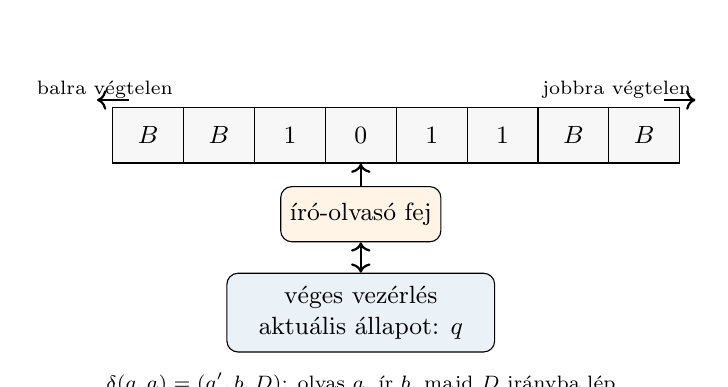
\begin{tikzpicture}[font=\small]
  \tikzset{cell/.style={draw, minimum width=9mm, minimum height=7mm, fill=black!3},
           head/.style={draw, rounded corners, fill=warnbg, minimum width=17mm, minimum height=7mm, align=center},
           ctrl/.style={draw, rounded corners, fill=lightaccent, minimum width=34mm, minimum height=10mm, align=center},
           lab/.style={font=\scriptsize}}

  \node[cell] (cell0) at (-2.7,0) {$B$};
  \node[cell] (cell1) at (-1.8,0) {$B$};
  \node[cell] (cell2) at (-0.9,0) {$1$};
  \node[cell] (cell3) at (0,0) {$0$};
  \node[cell] (cell4) at (0.9,0) {$1$};
  \node[cell] (cell5) at (1.8,0) {$1$};
  \node[cell] (cell6) at (2.7,0) {$B$};
  \node[cell] (cell7) at (3.6,0) {$B$};

  \node[lab] at (-3.25,0.58) {balra végtelen};
  \node[lab] at (3.25,0.58) {jobbra végtelen};
  \draw[->, thick] (-2.95,0.45) -- (-3.35,0.45);
  \draw[->, thick] (3.85,0.45) -- (4.25,0.45);

  \node[head] (h) at (0,-1.00) {író-olvasó fej};
  \draw[->, thick] (h.north) -- (cell3.south);
  \node[ctrl] (q) at (0,-2.25) {véges vezérlés\\aktuális állapot: $q$};
  \draw[<->, thick] (q.north) -- (h.south);
  \node[align=center, font=\scriptsize] at (0,-3.15) {$\delta(q,a)=(q',b,D)$: olvas $a$, ír $b$, majd $D$ irányba lép};
\end{tikzpicture}
\caption{Turing-gép szemléletes felépítése: szalag, fej és véges vezérlés}
\label{fig:zv10_turing_gep}
\end{figure}


Egy lépésben a gép:

\begin{enumerate}
  \item leolvassa a fej alatti jelet;
  \item az aktuális állapot és a leolvasott jel alapján új állapotba megy;
  \item felülírja a fej alatti cella tartalmát;
  \item a fejet balra, jobbra vagy bizonyos definíciókban helyben mozgatja.
\end{enumerate}

A szalagon a bemenet kezdetben egymás után szerepel, a többi cellában pedig az üres jel, gyakran $B$ vagy $\ast$, áll. A Turing-gép fontos sajátossága, hogy a memória nem közvetlenül címezhető: ha egy távoli cellát akar elérni, a fejnek lépésenként oda kell mozognia.

\subsection{Formális megadás}

Egy egyszerű, egyszalagos determinisztikus Turing-gép megadható például a következő adatokkal:
\[
  M=(K,\Sigma,\Gamma,\delta,q_0,B,F),
\]
ahol:

\begin{itemize}
  \item $K$ a belső állapotok véges halmaza;
  \item $\Sigma$ a bemeneti ábécé;
  \item $\Gamma$ a szalagábécé, amelyre $\Sigma\subseteq\Gamma$;
  \item $B\in\Gamma$ az üres jel, amely nem bemeneti jel;
  \item $q_0\in K$ a kezdőállapot;
  \item $F\subseteq K$ az elfogadó állapotok halmaza;
  \item $\delta$ az átmeneti függvény.
\end{itemize}

Az átmeneti függvény tipikus alakja:
\[
  \delta:K\times\Gamma \rightharpoonup K\times\Gamma\times\{L,R,S\}.
\]
A $\rightharpoonup$ jel azt fejezi ki, hogy a függvény lehet parciális. Ha például
\[
  \delta(q,a)=(q',b,R),
\]
akkor a gép $q$ állapotban $a$ jelet olvasva $q'$ állapotba megy, $b$ jelet ír az aktuális cellába, majd jobbra lép.

\begin{warningbox}
A Turing-gép nem azért állhat meg, mert elfogy a szalag. A szalag elvileg végtelen. A megállás oka az, hogy elér egy kijelölt végállapotot, vagy olyan konfigurációba jut, amelyre az átmeneti függvény nincs értelmezve.
\end{warningbox}

\section{A Turing-gép működése}

\subsection{Konfiguráció}

A Turing-gép pillanatnyi állapotát \textbf{konfigurációnak} nevezzük. Egy konfiguráció tartalmazza:

\begin{itemize}
  \item a szalag aktuális, lényeges tartalmát;
  \item az aktuális belső állapotot;
  \item a fej aktuális helyét.
\end{itemize}

Gyakori jelölés:
\[
  \alpha q \beta,
\]
ahol $\alpha$ a fej bal oldalán levő szalagrész, $q$ az aktuális állapot, $\beta$ pedig a fej alatti jellel kezdődő jobb oldali szalagrész. Ha $\beta$ első jele $a$, akkor a következő lépést a $\delta(q,a)$ átmenet határozza meg.

A kezdőkonfiguráció tipikusan:
\[
  q_0 w,
\]
ahol $w\in\Sigma^\ast$ a bemeneti szó, a fej pedig a bemenet első jelén áll. Ha az üres szó a bemenet, akkor a fej az első üres cellán áll.

\subsection{Számítási folyamat}

A \textbf{számítási folyamat} konfigurációk sorozata:
\[
  C_0,C_1,C_2,\ldots,
\]
ahol $C_0$ a kezdőkonfiguráció, és minden $C_{i+1}$ a $C_i$ konfigurációból egyetlen átmeneti lépéssel áll elő.

Egy számítás háromféleképpen viselkedhet:

\begin{itemize}
  \item \textbf{elfogad}: a gép elfogadó állapotban áll meg;
  \item \textbf{elutasít}: a gép nem elfogadó megállási állapotba jut, vagy explicit elutasító állapotot ér el;
  \item \textbf{nem áll meg}: a konfigurációk sorozata végtelen.
\end{itemize}

Ez utóbbi különösen fontos. A Turing-gép képes végtelen ideig futni, például ide-oda mozoghat két cella között, vagy mindig újabb üres cellák felé haladhat.

\subsection{Felismerés és eldöntés}

Egy Turing-gép \textbf{felismer} egy nyelvet, ha a nyelv szavait elfogadja. Olyan szavakra, amelyek nem tartoznak a nyelvbe, vagy elutasíthat, vagy akár végtelen ciklusba is kerülhet.

Egy Turing-gép \textbf{eldönt} egy nyelvet, ha minden bemenetre megáll, és pontosan a nyelv szavait fogadja el. Ez erősebb követelmény, mert nem engedi meg a nem megállást.

\begin{summarybox}
Felismerésnél az igen esetekben biztosan meg kell állni elfogadással, de a nem esetekben előfordulhat végtelen futás. Eldöntésnél minden bemeneten meg kell állni, és igen/nem választ kell adni.
\end{summarybox}

\subsection{Egyszerű példa: unáris növelés}

Tegyük fel, hogy a szalagon $1^n$ áll, vagyis $n$ darab egyes egymás után. A feladat az, hogy a gép írjon a végére még egy $1$ jelet, tehát az eredmény $1^{n+1}$ legyen.

\zvpseudocode[caption={Turing-gép szemléletű unáris növelés},label={lst:zv10_turing_unaris}]{src/code/zv10_turing_unaris_inkrementalas.pseudo}

A módszer lényege egyszerű: a gép jobbra mozog, amíg $1$ jeleket lát. Amikor eléri az első üres cellát, oda egy $1$ jelet ír, majd megáll. A példa azért hasznos, mert mutatja a Turing-gép alapvető működését: a távoli pozíció eléréséhez a fejnek végig kell lépkednie a szalagon.

\section{Univerzális Turing-gép és szimuláció}

\subsection{Az univerzalitás gondolata}

A Turing-gép eredeti szemléletben egy konkrét gép egy konkrét számítási feladathoz tartozik. A valódi számítógépek viszont programvezéreltek: ugyanaz a hardver sokféle programot képes futtatni.

Az \textbf{univerzális Turing-gép} ezt az ötletet formalizálja. Olyan Turing-gép, amely bemenetként megkapja egy másik Turing-gép leírását és annak bemenetét, majd szimulálja a leírt gép működését.

Szemléletesen:
\[
  U(\langle M\rangle,w)
\]
azt jelenti, hogy az $U$ univerzális gép az $M$ Turing-gép kódját és a $w$ bemenetet kapja meg, majd úgy viselkedik, mintha $M$ futna $w$-n.

\subsection{Miért fontos?}

Az univerzális Turing-gép jelentősége:

\begin{itemize}
  \item elméleti alapot ad a programvezérelt számítógép fogalmához;
  \item megmutatja, hogy a gép és a program elválasztható;
  \item lehetővé teszi, hogy gépek leírásairól mint adatokról beszéljünk;
  \item alapvető szerepe van az eldönthetetlenségi bizonyításokban, például a megállási probléma vizsgálatában.
\end{itemize}

A tétel szintjén elég azt érteni, hogy az univerzális gép nem új számítási erőt ad, hanem azt mutatja meg, hogy egyetlen rögzített gép megfelelő kódolással bármely másik Turing-gép működését tudja utánozni.

\section{A RAM-gép fogalma}

\subsection{Motiváció}

A Turing-gép matematikailag tiszta, de konkrét algoritmusok leírására kényelmetlen. Ha a fej egy távoli cellát akar elérni, lépésenként végig kell mennie a szalagon. A valódi számítógépek viszont címzett memóriával dolgoznak: egy memóriarekesz a címével közvetlenül elérhető.

A \textbf{RAM-gép}, azaz \emph{Random Access Machine}, ezt a szemléletet modellezi. Magyarul közvetlen elérésű gépnek is nevezhető.

\begin{figure}[htbp]
\centering
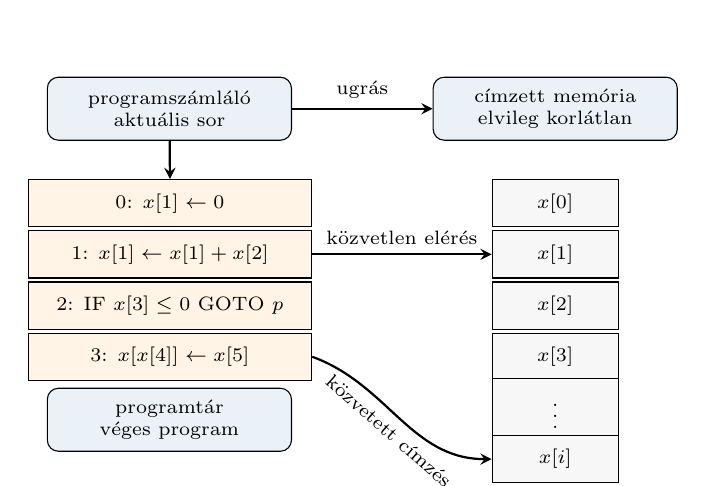
\begin{tikzpicture}[font=\scriptsize]
  \tikzset{box/.style={draw, rounded corners, fill=lightaccent, minimum width=31mm, minimum height=8mm, align=center},
           mem/.style={draw, fill=black!3, minimum width=16mm, minimum height=6mm, align=center},
           instr/.style={draw, fill=warnbg, minimum width=36mm, minimum height=6mm, align=left},
           arr/.style={->, >=stealth, thick}}

  \node[box] (pc) at (0,2.2) {programszámláló\\aktuális sor};
  \node[instr, anchor=west] (p0) at (-1.8,1.0) {0: $x[1]\leftarrow 0$};
  \node[instr, anchor=west] (p1) at (-1.8,0.35) {1: $x[1]\leftarrow x[1]+x[2]$};
  \node[instr, anchor=west] (p2) at (-1.8,-0.30) {2: IF $x[3]\leq 0$ GOTO $p$};
  \node[instr, anchor=west] (p3) at (-1.8,-0.95) {3: $x[x[4]]\leftarrow x[5]$};
  \node[box] (prog) at (0,-1.75) {programtár\\véges program};

  \node[mem] (m0) at (4.9,1.0) {$x[0]$};
  \node[mem] (m1) at (4.9,0.35) {$x[1]$};
  \node[mem] (m2) at (4.9,-0.30) {$x[2]$};
  \node[mem] (m3) at (4.9,-0.95) {$x[3]$};
  \node[mem] (md) at (4.9,-1.60) {$\vdots$};
  \node[mem] (mi) at (4.9,-2.25) {$x[i]$};
  \node[box] (memtitle) at (4.9,2.2) {címzett memória\\elvileg korlátlan};

  \draw[arr] (pc) -- (p0.north);
  \draw[arr] (p1.east) -- node[above] {közvetlen elérés} (m1.west);
  \draw[arr] (p3.east) to[out=-20,in=180] node[below, sloped] {közvetett címzés} (mi.west);
  \draw[arr] (pc.east) -- node[above] {ugrás} (memtitle.west);
\end{tikzpicture}
\caption{RAM-gép: programtár és közvetlenül címezhető memóriarekeszek}
\label{fig:zv10_ram_gep}
\end{figure}


\subsection{Felépítés}

A RAM-gép fő részei:

\begin{itemize}
  \item \textbf{programtár}: véges programot tartalmazó, sorokra bontott utasítássorozat;
  \item \textbf{memória}: elvileg végtelen sok, egész számmal címzett rekesz;
  \item \textbf{programszámláló}: megadja, hogy éppen melyik programsor hajtódik végre;
  \item \textbf{utasításkészlet}: egyszerű aritmetikai, értékadó és ugró utasítások.
\end{itemize}

A memóriarekeszeket gyakran így jelöljük:
\[
  x[0],x[1],x[2],\ldots
\]
A bemenet lehet például számok véges sorozata. Ilyenkor $x[0]$ tartalmazhatja a sorozat hosszát, $x[1],\ldots,x[n]$ pedig a bemeneti számokat.

\subsection{Tipikus utasítások}

Egy egyszerű RAM-modellben elegendő lehet például a következő utasítások használata:
\[
\begin{array}{lll}
  x[i]\leftarrow 0, & x[i]\leftarrow x[i]+1, & x[i]\leftarrow x[i]-1,\\
  x[i]\leftarrow x[i]+x[j], & x[i]\leftarrow x[i]-x[j], & \text{IF }x[i]\leq 0\text{ THEN GOTO }p.
\end{array}
\]

Fontos a \textbf{közvetett címzés} is:
\[
  x[x[i]]\leftarrow x[j],
  \qquad
  x[i]\leftarrow x[x[j]].
\]
Az első alak azt jelenti, hogy az $x[i]$ rekesz tartalma adja meg, melyik rekeszbe írunk. Ez a tömbök, mutatók és indexelt adatszerkezetek elméleti modellezéséhez hasznos.

\subsection{RAM példa: sorozat összege}

A következő pszeudókód azt mutatja, hogyan lehet a RAM-szemléletben egy bemeneti sorozat összegét kiszámítani. A bemenet hossza az $x[0]$ rekeszben van, az elemek az $x[1],\ldots,x[n]$ rekeszekben.

\zvpseudocode[caption={RAM-szemléletű összegzés közvetett memóriaeléréssel},label={lst:zv10_ram_osszegzes}]{src/code/zv10_ram_osszegzes.pseudo}

A példa nem egy konkrét gépi nyelv szintaxisa, hanem a RAM-modell gondolkodásmódját szemlélteti: rekeszek, indexek, közvetlen memóriaelérés és vezérlési feltétel jelenik meg benne.

\section{RAM költségmodell és kapcsolata a Turing-géppel}

\subsection{Egységköltségű és logaritmikus költségű RAM}

A RAM-modellben óvatosnak kell lenni az időméréssel. Ha minden utasítást egységnyi költségűnek tekintünk, akkor egyetlen lépésben akár nagyon nagy számokon is végezhetnénk műveletet. Ez elméletileg túl erős modellhez vezethet, mert nagy számokba sok információt lehet becsomagolni.

Két gyakori megközelítés:

\begin{itemize}
  \item \textbf{egységköltségű RAM}: minden alaputasítás költsége $1$;
  \item \textbf{logaritmikus költségű RAM}: egy művelet költsége arányos a benne szereplő címek és számok bitjeinek számával.
\end{itemize}

A logaritmikus költségű modell realisztikusabb, mert egy $m$ nagyságrendű szám leírásához körülbelül $\log_2 m$ bit kell. Ha tehát nagy számokkal dolgozunk, akkor a művelet költségét nem célszerű függetleníteni a számok hosszától.

\subsection{Turing-gép és RAM összehasonlítása}

\begin{center}
\begin{tabularx}{\textwidth}{L{40mm}L{42mm}X}
\toprule
\textbf{Szempont} & \textbf{Turing-gép} & \textbf{RAM-gép} \\
\midrule
Memória & Végtelen szalag cellákkal; a fej egyszerre egy cellát ér el. & Végtelen sok címzett memóriarekesz; tetszőleges rekesz közvetlenül címezhető. \\
Vezérlés & Véges állapothalmaz és átmeneti függvény. & Véges program gépi kód jellegű utasításokkal és ugrásokkal. \\
Egy lépés & Olvasás, írás, fejmozgatás, állapotváltás. & Egyszerű aritmetikai, értékadó, közvetett címzési vagy ugró utasítás. \\
Algoritmusleírás & Pontos, de konkrét algoritmusoknál nehézkes. & Gyakorlati algoritmusleíráshoz kényelmesebb. \\
Időmodell & Lépésszám, illetve szalaghasználat alapján elemezhető. & Egységköltségű vagy logaritmikus költségű RAM-modell használható. \\
Kiszámíthatóság & Univerzális modell; minden algoritmikusan kiszámítható függvény modellezésére alkalmas. & Lényegében ugyanazokat a függvényeket tudja kiszámítani; a különbség főleg a költségmodellben van. \\
\bottomrule
\end{tabularx}

\end{center}

A két modell közötti fő különbség a memóriaelérés. Turing-gépnél a fej lépésenként mozog, RAM-nál a címzett rekesz közvetlenül elérhető. Ennek ellenére kiszámíthatósági szempontból a két modell lényegében ekvivalens: amit az egyik ki tud számítani, azt megfelelő kódolással a másik is ki tudja számítani.

Bonyolultsági szempontból viszont megjelenhet szimulációs többlet. Egy Turing-gép RAM-on általában természetesen szimulálható, mert a szalag celláit memóriarekeszekbe lehet kódolni. Egy RAM-program Turing-gépen való szimulációja nehezebb, mert a Turing-gépnek meg kell keresnie a megfelelő című rekeszt a szalagon tárolt memóriaábrázolásban.

\begin{summarybox}
A vizsgán elég a fő gondolatot hangsúlyozni: a Turing-gép és a RAM-gép nem azért fontos, mert tényleges hardverleírások, hanem mert pontos számítási modellek. A Turing-gép elméletileg tiszta, a RAM pedig algoritmusleírásra kényelmesebb.
\end{summarybox}

\section{Boole-függvények}

\subsection{Definíció}

Egy $n$ változós \textbf{Boole-függvény} olyan leképezés, amely $n$ darab logikai értékből egy logikai értéket állít elő:
\[
  f:\{0,1\}^n\to\{0,1\}.
\]
Itt a $0$ értéket hamisnak, az $1$ értéket igaznak tekintjük. A változókat Boole-változóknak vagy logikai változóknak nevezzük.

Az $n$ változós Boole-függvények száma:
\[
  2^{2^n}.
\]
Ennek oka, hogy $n$ bemenet esetén $2^n$ különböző bemeneti sor van, és minden sorhoz kétféle kimeneti érték választható.

Például két változó esetén $2^{2^2}=16$ különböző Boole-függvény létezik.

\subsection{Alapműveletek}

\begin{center}
\begin{tabularx}{\textwidth}{L{24mm}L{24mm}L{28mm}X}
\toprule
\textbf{Művelet} & \textbf{Jelölés} & \textbf{Név} & \textbf{Mikor igaz?} \\
\midrule
Negáció & $\neg x$, $\overline{x}$ & NOT & Pont akkor igaz, ha $x$ hamis. \\
Konjunkció & $x\wedge y$ & AND, ÉS & Akkor igaz, ha mindkét bemenet igaz. \\
Diszjunkció & $x\vee y$ & OR, VAGY & Akkor igaz, ha legalább az egyik bemenet igaz. \\
Kizáró vagy & $x\oplus y$ & XOR & Akkor igaz, ha pontosan az egyik bemenet igaz. \\
Implikáció & $x\rightarrow y$ & HA $x$, AKKOR $y$ & Csak akkor hamis, ha $x$ igaz és $y$ hamis. \\
Ekvivalencia & $x\leftrightarrow y$ & XNOR & Akkor igaz, ha a két bemenet azonos értékű. \\
\bottomrule
\end{tabularx}

\end{center}

A leggyakoribb azonosságok:
\[
  \overline{\overline{x}}=x,
\]
\[
  x\wedge y=y\wedge x,
  \qquad
  x\vee y=y\vee x,
\]
\[
  x\wedge(y\vee z)=(x\wedge y)\vee(x\wedge z),
\]
\[
  x\vee(y\wedge z)=(x\vee y)\wedge(x\vee z).
\]

A De Morgan-azonosságok különösen fontosak:
\[
  \overline{x\wedge y}=\overline{x}\vee\overline{y},
  \qquad
  \overline{x\vee y}=\overline{x}\wedge\overline{y}.
\]

Ezek segítségével logikai kifejezéseket lehet átalakítani, egyszerűsíteni, illetve különböző kapukészletekre átírni.

\subsection{Igazságtábla}

Egy Boole-függvény teljesen megadható igazságtáblával. Például az XOR művelet:

\begin{center}
\begin{tabular}{ccc}
\toprule
$x$ & $y$ & $x\oplus y$ \\
\midrule
0 & 0 & 0 \\
0 & 1 & 1 \\
1 & 0 & 1 \\
1 & 1 & 0 \\
\bottomrule
\end{tabular}
\end{center}

Az XOR pontosan akkor igaz, ha a két bemenet különböző. Algebrai alakban:
\[
  x\oplus y=(\overline{x}\wedge y)\vee(x\wedge\overline{y}).
\]

\section{Normálformák}

\subsection{DNF és KNF}

A Boole-függvények többféle logikai formulával is felírhatók. A normálformák célja, hogy szabványos alakot adjanak.

\begin{center}
\begin{tabularx}{\textwidth}{L{28mm}L{35mm}X}
\toprule
\textbf{Fogalom} & \textbf{Felépítés} & \textbf{Jelentés} \\
\midrule
Literál & $x_i$ vagy $\overline{x_i}$ & Egy változó vagy annak negáltja. \\
Elemi konjunkció & Literálok konjunkciója & Egy konkrét bemeneti esetet vagy bemeneti esetek részhalmazát jelölhet. \\
DNF & Elemi konjunkciók diszjunkciója & A függvény igaz sorait írja le. Kanonikus alakban minden igaz sorhoz tartozik egy teljes minterm. \\
Elemi diszjunkció & Literálok diszjunkciója & Egy hamis bemeneti sor kizárására használható. \\
KNF & Elemi diszjunkciók konjunkciója & A függvény hamis sorait írja le. Kanonikus alakban minden hamis sorhoz tartozik egy teljes maxterm. \\
\bottomrule
\end{tabularx}

\end{center}

A \textbf{diszjunktív normálforma} olyan alak, amely elemi konjunkciók diszjunkciója. Igazságtáblából úgy állítható elő, hogy minden olyan sorhoz, ahol a függvény értéke $1$, felírunk egy konjunkciós tagot.

Ha például $f(x,y)$ csak a $(0,1)$ és $(1,0)$ sorokban igaz, akkor:
\[
  f(x,y)=(\overline{x}\wedge y)\vee(x\wedge\overline{y}).
\]
Ez éppen az XOR művelet.

A \textbf{konjunktív normálforma} elemi diszjunkciók konjunkciója. Igazságtáblából a hamis sorok alapján építhető fel.

\subsection{Teljesség}

Fontos tétel, hogy minden Boole-függvény felírható DNF-ben, ezért a $\neg$, $\wedge$, $\vee$ műveletek elegendőek minden Boole-függvény kifejezéséhez.

Más teljes kapukészletek is léteznek. Például önmagában a NAND vagy önmagában a NOR is funkcionálisan teljes, mert belőlük előállítható a negáció, az ÉS és a VAGY.

\section{Logikai hálózatok}

\subsection{Fogalom}

A \textbf{logikai hálózat} egy aciklikus irányított gráf, amely Boole-függvényt számít ki. A gráfban:

\begin{itemize}
  \item a forráscsúcsok a bemenetek;
  \item a belső csúcsok logikai kapuk;
  \item az élek a jelek továbbítását jelentik;
  \item a nyelőcsúcsok a kimenetek.
\end{itemize}

A hálózat aciklikus, mert a kapuk kimenete nem vezethet vissza olyan helyre, amelytől saját maga függne. Így a kapuk kiértékelhetők topologikus sorrendben: először a bemenetek értéke ismert, utána azok a kapuk számíthatók, amelyeknek minden bemenete ismert, és így tovább.

\begin{figure}[htbp]
\centering
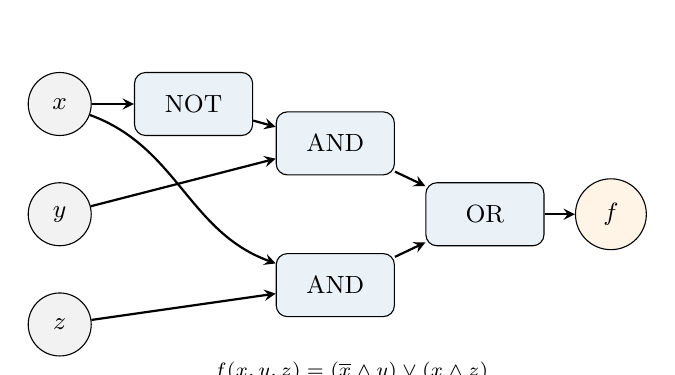
\begin{tikzpicture}[font=\small]
  \tikzset{inputnode/.style={draw, circle, fill=black!5, minimum size=8mm},
           gate/.style={draw, rounded corners, fill=lightaccent, minimum width=15mm, minimum height=8mm, align=center},
           outputnode/.style={draw, circle, fill=warnbg, minimum size=9mm},
           wire/.style={->, >=stealth, thick}}

  \node[inputnode] (x) at (0,1.4) {$x$};
  \node[inputnode] (y) at (0,0.0) {$y$};
  \node[inputnode] (z) at (0,-1.4) {$z$};

  \node[gate] (notx) at (1.7,1.4) {NOT};
  \node[gate] (and1) at (3.5,0.9) {AND};
  \node[gate] (and2) at (3.5,-0.9) {AND};
  \node[gate] (or1) at (5.4,0.0) {OR};
  \node[outputnode] (f) at (7.0,0.0) {$f$};

  \draw[wire] (x) -- (notx);
  \draw[wire] (notx) -- (and1);
  \draw[wire] (y) -- (and1);
  \draw[wire] (x) to[out=-20,in=160] (and2);
  \draw[wire] (z) -- (and2);
  \draw[wire] (and1) -- (or1);
  \draw[wire] (and2) -- (or1);
  \draw[wire] (or1) -- (f);

  \node[align=center, font=\scriptsize] at (3.7,-2.0) {$f(x,y,z)=(\overline{x}\wedge y)\vee(x\wedge z)$};
\end{tikzpicture}
\caption{Egyszerű aciklikus logikai hálózat egy Boole-függvény kiszámítására}
\label{fig:zv10_logikai_halozat}
\end{figure}


Az ábrán látható hálózat a következő függvényt számítja ki:
\[
  f(x,y,z)=(\overline{x}\wedge y)\vee(x\wedge z).
\]

\subsection{Méret és mélység}

A logikai hálózat két fontos mértéke a \textbf{méret} és a \textbf{mélység}.

\begin{center}
\begin{tabularx}{\textwidth}{L{30mm}L{30mm}X}
\toprule
\textbf{Mérték} & \textbf{Jelentés} & \textbf{Miért fontos?} \\
\midrule
Méret & A kapuk száma, gyakran $s(H)$. & A teljes elvégzendő munkát, illetve a hardverigényt közelíti. \\
Mélység & A leghosszabb bemenettől kimenetig vezető út hossza, gyakran $d(H)$. & A párhuzamos időt szemlélteti, mert egy szint kapui elvileg egyszerre számíthatók. \\
Befok & Egy kapu bemeneteinek száma. & Nagy befok erős kaput jelenthet; gyakran korlátozzuk például legfeljebb kettőre. \\
Kifok & Egy csúcs kimenetének felhasználási száma. & Ha korlátlan, akkor egy kiszámított bit sok helyre ingyen továbbadható; valós hardvernél ez nem mindig reális. \\
\bottomrule
\end{tabularx}

\end{center}

A \textbf{méret} általában a kapuk száma. Ez azt mutatja, hogy mennyi elemi művelet vagy hardverelem szükséges.

A \textbf{mélység} a leghosszabb bemenettől kimenetig vezető út hossza. Ez párhuzamos végrehajtás szempontjából fontos, mert azonos szinten levő, egymástól független kapuk egyszerre számolhatók. Ha egy hálózat mérete $s$, mélysége $d$, akkor egy processzorral nagyjából $O(s)$ művelet kell, sok párhuzamos végrehajtó egységgel pedig ideális esetben a mélység adja a kritikus utat.

\subsection{Kapuáramkör és Boole-polinom kapcsolata}

Egy logikai formula felfogható fa alakú logikai hálózatként. Például az
\[
  (\overline{x}\wedge y)\vee(x\wedge z)
\]
formula egy olyan hálózatot ad, ahol a részformulák kapukként jelennek meg.

A logikai hálózat ennél általánosabb, mert egy már kiszámított részeredményt több későbbi kapu is felhasználhat. Ez gyakran rövidebb vagy kisebb hálózatot eredményezhet, mint ha ugyanazt a részformulát többször külön felírnánk.

\subsection{Félösszeadó példa}

A félösszeadó két bitet ad össze. Bemenetei $x$ és $y$, kimenetei:

\begin{itemize}
  \item $s$: összegbit;
  \item $c$: átviteli bit.
\end{itemize}

A függvények:
\[
  s=x\oplus y,
  \qquad
  c=x\wedge y.
\]

Igazságtáblája:

\begin{center}
\begin{tabular}{cccc}
\toprule
$x$ & $y$ & $c$ & $s$ \\
\midrule
0 & 0 & 0 & 0 \\
0 & 1 & 0 & 1 \\
1 & 0 & 0 & 1 \\
1 & 1 & 1 & 0 \\
\bottomrule
\end{tabular}
\end{center}

Ez jól mutatja, hogy a logikai hálózatok nemcsak elméleti modellek, hanem digitális áramkörök leírására is használhatók.

\section{A három modell kapcsolata}

\subsection{Közös szemlélet}

Mindhárom modell ugyanazt a kérdést vizsgálja: hogyan lehet formálisan leírni egy számítást?

\begin{itemize}
  \item A \textbf{Turing-gép} a számítást lépésenként, szalagon mozgó fejjel írja le.
  \item A \textbf{RAM-gép} a számítást programként és címzett memóriarekeszek műveleteként írja le.
  \item A \textbf{logikai hálózat} a számítást Boole-kapuk aciklikus függőségi gráfjaként írja le.
\end{itemize}

A Turing-gép és a RAM-gép általános modell: különböző hosszúságú bemenetekre is ugyanaz a gép vagy program fut. A logikai hálózatnál viszont a bemenethossz rögzített. Ha minden $n$ bemenethosszra külön hálózatot adunk, akkor hálózatcsaládról beszélhetünk.

\subsection{Szimulációs gondolat}

A modellek közötti kapcsolat megérthető szimulációval:

\begin{itemize}
  \item Turing-gép szimulálható RAM-on: a szalag celláit memóriarekeszekbe kódoljuk, a fej pozícióját és az állapotot külön rekeszben tároljuk.
  \item RAM-program szimulálható Turing-gépen: a memóriarekeszek tartalmát a szalagon kell tárolni és keresni.
  \item Rögzített ideig futó, rögzített bemenethosszú Turing-gép működése logikai hálózattal is leírható, mert minden időpillanat és szalagpozíció állapota Boole-változókkal kódolható.
\end{itemize}

A szimulációk gyakran többletidőt vagy többletméretet okoznak, de elméletileg azt mutatják, hogy a modellek között mély kapcsolat van.

\section{Gyakori félreértések}

\subsection{A Turing-gép nem fizikai gépterv}

A Turing-gép nem egy modern processzor modellje, hanem absztrakt matematikai eszköz. Nem az a célja, hogy hardveresen hatékony legyen, hanem hogy pontosan megfoghatóvá tegye az algoritmikus számítás fogalmát.

\subsection{A RAM-gép végtelen memóriája idealizáció}

A RAM-gép memóriája elvileg korlátlan, és a rekeszek tetszőleges nagy számokat is tartalmazhatnak. Ez nem valós hardverállítás, hanem matematikai egyszerűsítés. Ezért kell figyelni arra, hogy milyen költségmodellt választunk.

\subsection{A logikai hálózat nem ugyanaz, mint egy ciklust tartalmazó program}

A logikai hálózat aciklikus. Nincs benne ciklus, ezért rögzített számú kapukiértékeléssel eredményt ad. Egy általános program ciklusokat, rekurziót és változó futási időt is tartalmazhat, ezért általánosabb, mint egyetlen rögzített logikai hálózat.

\section{Tipikus vizsgakérdések és rövid válaszvázlatok}

\subsection{Mi a Turing-gép?}

Véges vezérléssel, szalaggal és író-olvasó fejjel rendelkező absztrakt gép. Egy lépésben állapot és olvasott jel alapján ír, állapotot vált és mozgatja a fejet.

\subsection{Mit jelent a konfiguráció?}

A gép pillanatnyi teljes leírása: a lényeges szalagtartalom, az aktuális állapot és a fej pozíciója.

\subsection{Mi a különbség felismerés és eldöntés között?}

Felismerésnél a nyelv szavait a gép elfogadja, de a nyelven kívüli szavakon futhat végtelenül. Eldöntésnél minden bemeneten meg kell állnia, és helyes igen/nem választ kell adnia.

\subsection{Mi a RAM-gép fő előnye a Turing-géphez képest?}

A közvetlen memóriaelérés. A RAM-gép rekeszeket címez, ezért konkrét algoritmusok leírására közelebb áll a valós programozási szemlélethez.

\subsection{Miért kell logaritmikus költségű RAM-modell?}

Mert nagy számokkal végzett műveletek egységköltségűnek vétele irreálisan erős modellhez vezethet. Logaritmikus költségnél a számok bitmérete is beleszámít az időbe.

\subsection{Mi a Boole-függvény?}

Olyan függvény, amely $n$ darab $0/1$ bemenetből egy $0/1$ kimenetet számít:
\[
  f:\{0,1\}^n\to\{0,1\}.
\]

\subsection{Mi a logikai hálózat?}

Aciklikus irányított gráf, amelyben a bemenetekből logikai kapukon keresztül kimeneteket számítunk. A kapuk Boole-függvényeket valósítanak meg.

\subsection{Mit jelent a hálózat mérete és mélysége?}

A méret a kapuk száma, a mélység a leghosszabb bemenettől kimenetig vezető út hossza. A méret a teljes munkát, a mélység a párhuzamos kritikus utat szemlélteti.

\section{Összefoglalás vizsgára}

Rövid, vizsgán jól használható összefoglalás:

\begin{itemize}
  \item A számítási modell célja az algoritmus fogalmának pontosítása.
  \item A Turing-gép véges vezérlésből, szalagból, író-olvasó fejből és átmeneti függvényből áll.
  \item Egy Turing-lépés: olvasás, írás, állapotváltás, fejmozgatás.
  \item A konfiguráció a teljes pillanatnyi gépállapotot írja le.
  \item A Turing-gép megállhat elfogadással, elutasítással, vagy futhat végtelen ideig.
  \item Felismerésnél a nemleges esetekben megengedett a nem megállás; eldöntésnél minden bemeneten meg kell állni.
  \item Az univerzális Turing-gép más Turing-gépek leírását programként kezeli és szimulálja.
  \item A RAM-gép programtárból és közvetlenül címezhető memóriarekeszekből áll.
  \item A RAM konkrét algoritmusok leírására kényelmesebb, mint a Turing-gép, de a költségmodellre figyelni kell.
  \item Egységköltségű RAM-nál minden alaputasítás ára $1$; logaritmikus költségnél a számok és címek bithossza is számít.
  \item A Turing-gép és a RAM-gép kiszámíthatósági értelemben lényegében ekvivalens.
  \item A Boole-függvény $f:\{0,1\}^n\to\{0,1\}$ alakú logikai függvény.
  \item Az $n$ változós Boole-függvények száma $2^{2^n}$.
  \item Minden Boole-függvény felírható DNF-ben, ezért a $\neg,\wedge,\vee$ műveletek elegendőek.
  \item A logikai hálózat aciklikus irányított gráf, amely kapukkal számít ki Boole-függvényt.
  \item A hálózat mérete a kapuk száma, mélysége a leghosszabb függőségi lánc hossza.
  \item A logikai hálózat rögzített bemenethosszú modell; általános feladatokhoz hálózatcsaládokkal dolgozunk.
\end{itemize}

\end{document}
